
\section{系统设计方案}

\subsection{设计目标与需求分析}

\subsubsection{设计目标}

针对第二章归纳的研究不足，本文系统设计围绕“规划与数据一致、知识约束可控、执行流程可落地、结论生成可迭代”四个目标展开。上述目标并非彼此孤立，而是共同构成系统从问题输入到结论输出的整体设计原则。其中，前两个目标主要回答“系统应当如何做出较好的分析决策”，后两个目标则进一步回答“这些决策如何被稳定执行并持续优化”。因此，设计目标既体现方法层面的研究诉求，也体现原型系统层面的工程约束。

第一，数据感知目标。系统在任务规划前必须读取并理解当前数据集关键特征，包含列类型分布、变量统计关系、图结构特征和代表性文本样本，避免“先规划后看数”的常见倒置流程。这一目标的核心在于，让规划阶段不再仅依赖用户问题表述和通用经验，而是建立在对当前数据事实的显式感知之上。对于专利分析场景而言，不同数据集在字段完备性、时间跨度、技术分类粒度、引文网络规模和文本语义密度等方面往往差异显著，因此系统必须先识别“数据中有什么、能支持什么、存在什么限制”，再决定“应该如何分析”。

第二，知识增强目标。系统需要显式引入领域知识约束，但约束形式不能是单一模板化硬编码。本文采用因果图谱与方法图谱协同机制：前者约束“研究假设合理性”，后者约束“分析方法可执行性”\cite{pan2024unifying,liu2016knowledge}。该目标强调，系统既不能完全放任大语言模型自由生成分析路径，也不能把领域经验固化为僵化模板，而应通过结构化知识提供“可引导、可组合、可扩展”的约束机制。这样既能够提升方案的理论一致性，又能保留一定的探索空间，以适配复杂且异质的专利分析问题。

第三，迭代优化目标。复杂专利问题往往无法在单轮规划中获得充分证据，系统需支持基于第一轮执行结果自动修正和深化分析路径，形成“探索—验证”的双轮机制。该目标对应真实研究过程中的渐进式分析特点，即初始分析通常只能识别主效应与显著信号，而更深入的机制解释、边界条件识别和稳健性验证往往依赖于前一轮的执行反馈。因此，系统设计不能停留在一次性输出方案的层面，而应支持基于结果回流进行二次规划与差距修补。

第四，端到端闭环目标。系统不仅要输出规划文本，还要保证方案可被转化为技术规格、可执行代码和最终报告，实现从用户问题到分析结论的完整自动化链路\cite{hong2024metagpt,langgraph2024}。这一目标强调系统设计必须兼顾“研究方案生成”与“工程流程闭环”两方面要求，避免出现规划结果看似合理、但无法被稳定执行和复核的情况。只有当规划、规格化、执行、评审与结果沉淀形成闭环时，系统才真正具备可复现、可追踪和可部署的应用价值。

\subsubsection{功能需求}

基于上述目标，系统的功能需求可分为四个层次。这些需求从前端的数据理解能力，逐步延伸到中间的方案规划与执行能力，再到末端的结果评审与过程留痕能力，共同构成系统原型的核心功能边界。

\textbf{数据感知需求。}系统需支持自动解析 Excel 格式的专利数据集，识别列语义类型（数值、分类、日期、文本、多值分隔符列），计算跨列统计关系（相关系数、分组对比、时间趋势），并从多值字段自动构建图结构（共现网络、合作网络、引用网络）。这一需求的关键不只是“读入数据”，而是形成对数据整体结构的初步画像，为后续规划提供可直接调用的事实基础。

\textbf{方案规划需求。}系统需基于数据事实和领域知识生成结构化分析蓝图。蓝图采用有向无环图（DAG）表示。每个任务节点包含明确的研究问题、输入输出变量、方法选择和参数配置。蓝图需通过拓扑排序验证依赖合法性，并通过列名校验保证数据可用性。该需求确保系统输出的不是松散建议，而是可以被后续执行模块直接消费的结构化方案。

\textbf{自动执行需求。}系统需将蓝图自动转化为可执行的 Python 分析代码，在沙箱环境中运行并捕获结果。当执行失败时，需根据错误信息自动修复并重试。对于自动化分析系统而言，执行能力不仅决定方案能否真正落地，也决定系统是否能够在现实数据环境中应对列名偏差、类型不匹配和外部库调用异常等常见问题。
\textbf{质量保证需求。}系统需对执行结果进行结构完整性检查和语义有效性评估，确保输出结果回答了研究问题。同时，所有中间产物（蓝图 JSON、技术规格、代码、执行结果）需持久化存储，支持事后复核。该需求对应系统的可信性要求，即不仅要“生成结果”，还要使结果具备可解释、可追溯和可审计的特征。

\subsubsection{非功能需求}

\textbf{可复现性。}同一数据集与研究问题在相同配置下应产出结构一致的分析方案。关键随机过程（如抽样、社区检测）使用固定随机种子。该要求保证实验结果和系统行为能够被稳定复核，避免因流程波动过大而削弱结论可信度。

\textbf{可扩展性。}系统架构应支持新增分析场景而无需修改核心流程。具体而言，新的研究问题类型只需通过因果图谱和方法图谱的扩展来支持，不需要修改智能体代码。该要求体现本文系统面向长期演化的设计思路，即通过扩充知识资源而非频繁重写流程逻辑来支持新任务。

\textbf{性能约束。}数据感知阶段（DataPreview + GraphPreview）应在 30 秒内完成，避免规划前预处理成为瓶颈。大规模图（节点数超过 10,000）需自动降级算法复杂度。该要求保证系统在实际应用中具备可接受的响应效率，避免因前置分析开销过大而削弱整体可用性。

\subsection{总体方案框架}

\subsubsection{四智能体流水线架构}

本文采用四智能体流水线架构，主体由 Strategist、Methodologist、CodingAgent、Reviewer 组成，工作流由 LangGraph 状态机编排\cite{langgraph2024}。系统总体架构如图 3-1 所示。之所以采用“四智能体串联”的组织方式，而非单智能体直接完成全部任务，主要是因为专利分析方案生成本质上属于一个跨越“研究规划、方法规格化、代码执行、结果评审”多个认知层级的复合任务。若将上述职责全部交由单一智能体承担，往往会导致规划深度不足、执行细节混乱以及结果解释不稳定等问题；而通过角色分工，可以将不同阶段的目标、输入输出形式和质量标准显式拆开，从而提高系统整体的稳定性与可控性。

在该架构中，四个智能体并非简单顺序调用关系，而是构成一个具有明确职责边界的闭环流水线。前端的 Strategist 负责把用户问题、数据事实和领域知识整合为“应当做什么”的分析蓝图；中间的 Methodologist 负责将蓝图进一步转化为“如何精确执行”的技术规格；后端的 CodingAgent 则完成“将方案落地为可执行代码并获取结果”的过程；最终由 Reviewer 对执行结果进行质量审查和结论整合，形成可直接面向用户输出的分析结果。通过这样的分层设计，系统能够把高层研究意图与底层执行实现解耦，减少单一阶段错误向全流程扩散的风险。

% 图3-1
\begin{figure}[htbp]
\centering
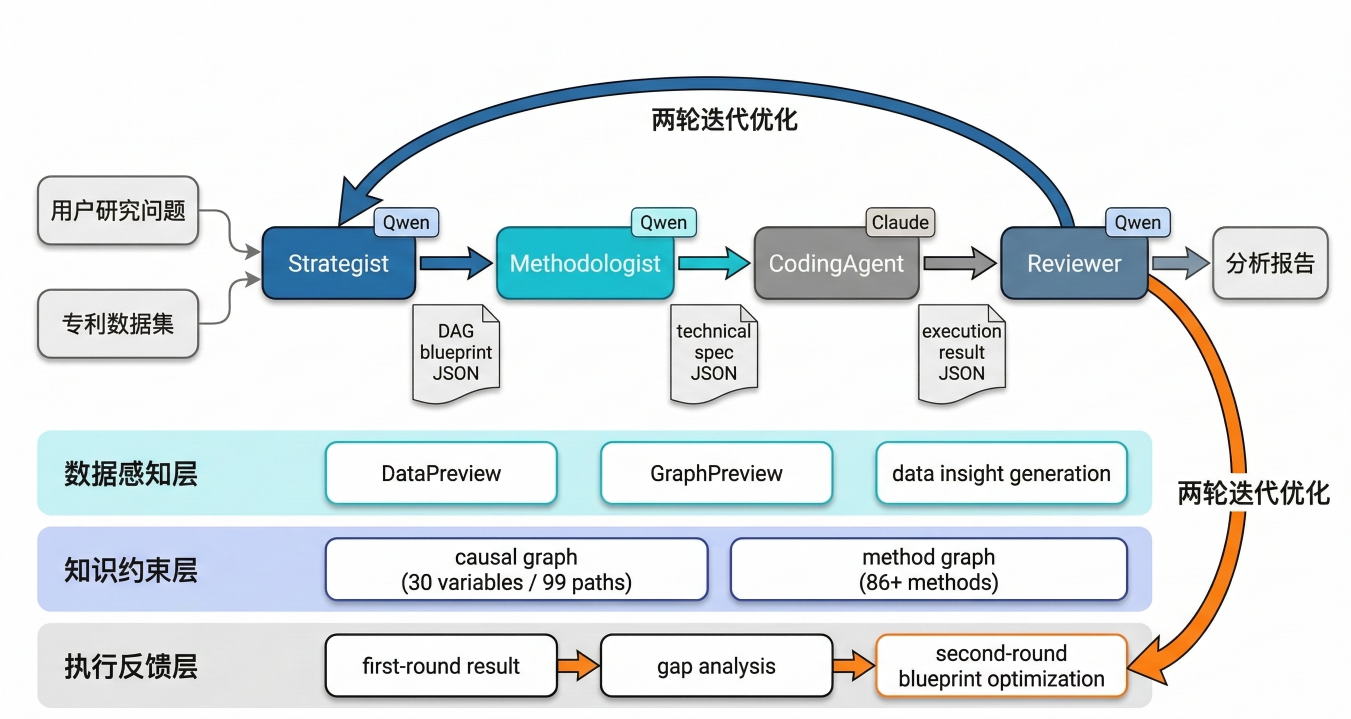
\includegraphics[width=0.95\textwidth]{figures/new_img/图3-1.png}
\caption{系统总体架构图}
\label{fig:3-1}
\end{figure}

各智能体职责与输入输出如下：

\begin{enumerate}[(1)]
\item Strategist（规划智能体）：接收用户研究问题，调用数据感知模块与双图谱模块，输出结构化 DAG 分析蓝图。蓝图节点包括任务目标、输入输出变量、方法建议和参数配置。该智能体是系统的核心决策者，其输出质量直接决定后续分析深度。换言之，Strategist 主要承担“研究设计者”的角色，负责在多种可行路径中选择最值得执行的分析主线。
\item Methodologist（方法规格化智能体）：将蓝图节点进一步规格化，生成可执行技术说明，包括函数签名、输入契约、变量约束、参数要求与预期输出类型。该智能体充当规划层与执行层之间的“翻译器”，将高层研究意图转化为精确的技术合同。其存在的意义在于避免 CodingAgent 直接面对过于抽象的规划描述，从而降低代码生成阶段的歧义与偏差。
\item CodingAgent（执行智能体）：基于规格自动生成 Python 分析代码并在沙箱环境中执行；若执行失败（如列名不存在、类型错误、统计包调用异常），利用错误反馈进行迭代修复，最多重试 15 轮。该智能体承担的是“工程实现者”角色，其核心任务并非仅仅写出代码，而是确保分析任务能够在真实数据环境中被稳定执行并返回结构化结果。
\item Reviewer（评审智能体）：对执行结果进行结构一致性检查与语义有效性评估，生成最终分析报告并返回关键证据链。该智能体相当于系统中的“质量把关者”，负责判断执行结果是否真正回答了原始研究问题，以及当前证据是否足以支撑相应结论。
\end{enumerate}

在智能体选型上，系统采用“双模型分工”策略：通义千问（Qwen）负责文本规划与评审任务（Strategist、Methodologist、Reviewer），Claude 负责代码生成与执行修复任务（CodingAgent）\cite{zhao2024llm,brown2020language}。这一设计并非简单叠加多个模型，而是基于不同模型在长文本理解、结构化规划、代码生成与错误修复等方面的能力差异进行功能匹配。前者更适合处理研究问题理解、方法组织与结果总结等偏语言规划任务，后者更适合处理程序生成、报错修复和执行迭代等偏工程实现任务。该组合将“文本规划稳定性”和“代码生成准确性”分别优化，降低单模型在全流程任务中的能力短板，也使系统在整体上具备更好的鲁棒性与任务适配能力。

\subsubsection{三个基础能力层}

在智能体链路之外，系统包含三个基础能力层。若将四智能体流水线理解为系统的“决策与执行主体”，那么这三个能力层则构成其稳定运行所依赖的底层支撑环境。它们分别从数据事实供给、领域知识约束和执行结果回流三个方面，为智能体链路提供输入依据、边界条件和迭代动力。这样的设计避免了智能体仅凭自然语言上下文完成复杂分析规划，也使系统从“模型驱动”进一步转向“模型 + 数据 + 知识 + 反馈”共同驱动。

\textbf{数据感知层}：DataPreview 与 GraphPreview 分别处理统计关系与图结构关系，输出结构化事实。DataPreview 负责列类型识别、跨列相关系数计算、分组对比和时间趋势检测；GraphPreview 负责自动检测多值字段、构建图结构并运行标准图算法（社区检测、中心性分析等）。两个模块的输出合并后驱动 LLM 生成“数据洞察”，为蓝图规划提供证据基础。该能力层解决的是“系统如何在规划前理解当前数据”的问题，其价值在于将原本隐含在原始表格和网络结构中的信息显式化、结构化，从而使后续智能体能够围绕真实数据特征而不是抽象问题描述开展分析。

\textbf{知识约束层}：因果图谱编码了专利计量领域的核心变量关系（30 个变量、99 条因果路径），提供假设生成的 6 种策略模板；方法图谱包含 86 种以上分析方法，提供变量测量和统计分析的推荐方案。两类图谱均基于 Web of Science 检索获取的 800 余篇专利分析领域文献，经系统性编码提取而成（详见第四章 4.2.6 节）。两类图谱在 Strategist 阶段协同使用：先由因果图谱确定“研究什么”，再由方法图谱确定“怎么做”\cite{pan2024unifying,liu2016knowledge}。该能力层解决的是“系统如何避免规划完全依赖语言模型自由生成”的问题，通过将领域经验、变量关系和方法路径组织为可调用的结构知识，为分析方案提供理论边界与方法指引。

\textbf{执行反馈层}：第一轮执行结果经差距分析后回流 Strategist，用于第二轮蓝图优化。差距分析自动评估第一轮“已回答”和“未充分回答”的问题，并提出深化策略（如增加控制变量、引入非线性模型、补充机制检验等）。该能力层解决的是“系统如何根据实际结果持续修正方案”的问题，使整个工作流不再停留于一次性规划，而具备基于执行证据进行自我修补和逐步深化的能力。

从整体关系看，数据感知层提供“事实输入”，知识约束层提供“结构边界”，执行反馈层提供“修正依据”。三者共同嵌入四智能体流水线之中，使系统在前端具备感知能力，在中端具备约束能力，在后端具备学习式优化能力。这种设计使得系统总体上不只是一个多智能体协作框架，而是一个具备数据支撑、知识支撑与反馈支撑的分析决策系统。

\subsubsection{模块间数据流}

从“用户输入研究问题”到“系统输出分析报告”，整体流程被组织为一条单向流水线，各模块间通过结构化 JSON 传递信息，既保证了链路的清晰可视，又便于在任意阶段插入人工检查或替换实现模块。

\begin{enumerate}[(1)]
\item 用户输入研究问题（字符串）和数据文件路径后，DataPreview 和 GraphPreview 并行处理数据集，分别输出统计摘要文本和图结构特征文本。该步骤完成的是对原始数据的“感知与表征”，将难以直接纳入提示词的大规模表格与网络，压缩为可被 LLM 理解的结构化事实输入。
\item Strategist 接收上述文本、用户目标和双图谱查询结果，输出 DAG 蓝图 JSON。蓝图中每个任务节点的 \texttt{columns\_to\_load} 字段经过列名校验，确保引用的列在数据集中实际存在。此时系统完成了从“研究问题 + 数据事实 + 领域知识”到“可执行任务图”的映射，为后续自动化实现提供清晰的任务分解和依赖关系。
\item Methodologist 逐个接收蓝图节点，输出技术规格 JSON。技术规格包含函数签名、输入验证逻辑和预期输出结构，起到“自然语言规划”和“可执行代码”之间的中间契约作用，使 CodingAgent 可以在不反复理解上游语义的前提下，专注于代码生成与调试。
\item CodingAgent 基于技术规格生成 Python 代码并执行，输出结果 JSON 文件。若执行失败，错误信息反馈给 CodingAgent 触发修复循环。该阶段将抽象分析任务具体化为脚本级操作，并通过自动修复机制提高执行成功率，减少因代码错误导致的整条流水线中断。
\item Reviewer 接收所有任务的执行结果，输出评审报告。在两轮迭代模式下，第一轮的评审结果和原始执行输出反馈给 Strategist，驱动第二轮蓝图生成，使系统具备在“规划—执行—评审”闭环内自我迭代的能力。
\end{enumerate}

该流水线模式的关键优势是\textbf{中间产物完全可追踪}：蓝图 JSON、技术规格、Python 代码和执行结果均有独立文件，便于事后审计和复跑验证\cite{hong2024metagpt}。此外，由于每一阶段均采用明确的数据结构进行输入输出，系统可以在不改动整体架构的前提下替换局部实现（如更换 LLM 或执行环境），增强了工程上的可维护性与可扩展性。

\subsection{数据感知方案生成流程}

本节阐述系统的核心创新——数据感知方案生成的设计思路。

传统 LLM 分析系统的规划过程为"问题$\rightarrow$方案"，即仅根据问题语义生成分析任务，不考虑当前数据集的具体特征。该模式的主要问题是方案容易模板化——对不同数据集生成高度相似的分析路径\cite{guo2024dsagent,hong2025data}。

本文提出的数据感知流程将规划过程改为"问题 + 数据事实$\rightarrow$洞察$\rightarrow$方案"，如图 3-2 所示。

% 图3-2
\begin{figure}[htbp]
\centering
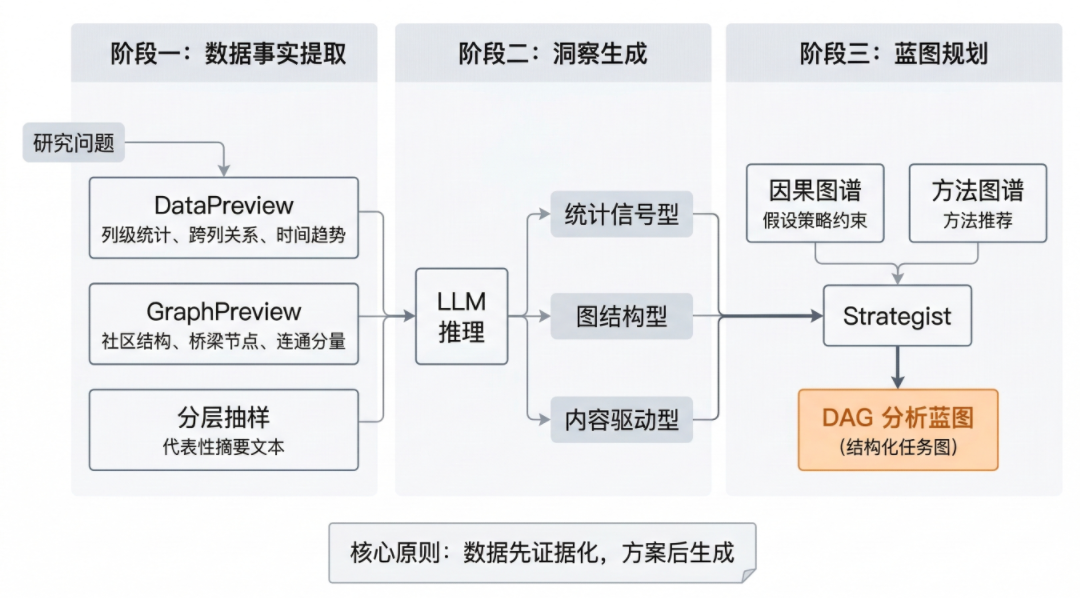
\includegraphics[width=0.95\textwidth]{figures/new_img/图3-2.png}
\caption{数据感知方案生成流程图}
\label{fig:3-2}
\end{figure}

具体分为三个阶段：

\textbf{阶段一：数据事实提取}。DataPreview 提取列级统计和跨列关系（相关系数、分组均值差异、时间趋势），GraphPreview 提取网络结构特征（社区、桥梁节点、连通分量），分层抽样提供代表性摘要文本。该阶段的输出是纯粹的结构化事实，不包含任何语义解读。
  
\textbf{阶段二：洞察生成}。将阶段一的三类输出（统计特征、图结构、摘要样本）合并为 LLM 提示词，驱动 LLM 生成可检验的研究洞察。每条洞察包含具体的数据观察（必须引用数字）、可检验假设、涉及列名和建议方法。洞察分为统计信号型、图结构型和内容驱动型三类。
  
\textbf{阶段三：蓝图规划}。Strategist 以洞察为主驱动、以双知识图谱为辅助约束，生成 DAG 蓝图。该阶段选择 2-3 条核心洞察作为分析起点，结合因果图谱的假设策略和方法图谱的方法推荐，设计具体的分析任务链。

该过程的核心设计原则是\textbf{数据先证据化、方案后生成}：系统先将数据转化为结构化证据，再基于证据设计方案，而非反过来。

\subsection{两轮迭代优化设计}

在前述多智能体架构与基础能力层之上，系统进一步引入两轮迭代优化机制，将整体行为从"一次性生成"改为"反馈驱动生成"，整体流程如图 3-3 所示。该机制的核心思想是把传统实证研究中"探索—验证"的两阶段范式显式编码进自动化流水线，使系统能够围绕首轮结果进行针对性深化，而非简单重复同类分析。

% 图3-3
\begin{figure}[htbp]
\centering
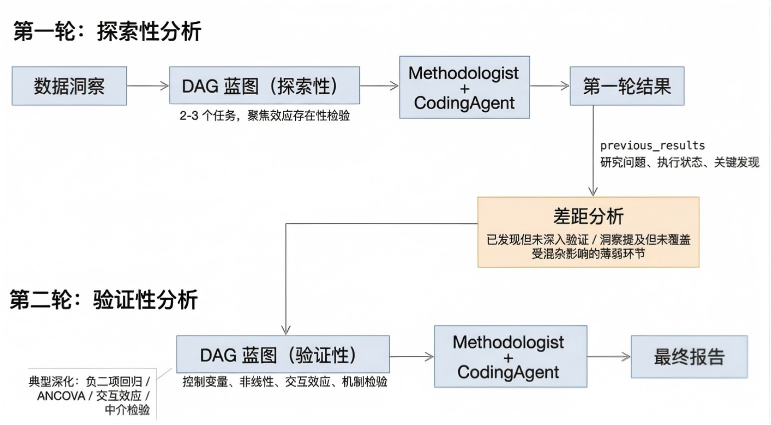
\includegraphics[width=0.95\textwidth]{figures/new_img/图3-3.png}
\caption{两轮迭代优化流程图}
\label{fig:3-3}
\end{figure}

设计思路如下：

\textbf{第一轮（探索性分析）}：基于数据洞察生成初始 DAG 蓝图，通常包含 2-3 个任务，聚焦效应存在性检验（如"X 是否显著影响 Y"）。该轮的目标是快速建立基础变量关系图谱并发现初步信号，为后续集中资源在"最有前景的关系"上提供筛选依据。

\textbf{中间环节（差距分析）}：系统自动评估第一轮结果，识别三类缺口：（1）已发现但未深入验证的信号；（2）洞察中提及但第一轮未覆盖的分析方向；（3）第一轮结论可能受混杂因素影响的薄弱环节。差距分析结果形成第二轮的规划约束，从而避免第二轮重新"从零规划"，而是围绕已发现的问题链路进行有约束的深化。

\textbf{第二轮（验证性分析）}：基于差距分析生成深化 DAG 蓝图，通常引入更多控制变量、非线性模型（如负二项回归替代 OLS）、交互效应检验或机制路径分析（如中介效应检验）。该轮的目标是将分析从"效应是否存在"提升至"效应的机制、路径和边界条件"，使最终结论在因果解释力度和稳健性上更接近实证研究常规标准。

两轮之间的信息传递通过 \texttt{previous\_results} 参数实现，包含第一轮各任务的研究问题、执行状态和关键发现。该方法确保第二轮方案基于第一轮的实际证据而非预设假设。

选择两轮而非单轮或更多轮的设计依据如下。首先，从科学研究方法论角度，"探索—验证"的两阶段范式是实证研究的经典结构：第一阶段建立初步假设并收集证据，第二阶段在控制混杂变量的条件下验证和深化假设\cite{basberg1987patents,trajtenberg1990penny}。该结构既避免了单轮分析因缺乏反馈而产生的浅层化问题，也避免了过多轮次导致的分析主题发散。其次，从边际收益角度，第一轮通常覆盖最显著的变量关系和主效应，第二轮基于差距分析引入控制变量、非线性检验和机制验证，分析层次从"效应发现"提升至"机制解释"。

若引入第三轮，新增信息的边际贡献将显著递减，因为核心假设和主要变量关系已在前两轮中被充分探索。最后，从工程成本角度，每轮涉及 LLM 规划调用、代码生成与执行、结果评审等完整流水线，计算开销随轮次线性增长，两轮在分析深度与资源消耗之间取得了合理平衡。

\subsection{典型应用场景映射}

为验证系统通用性，本文选取三类专利计量场景作为标准应用模板，覆盖“因果效应识别—结构与演化—跨主体比较”三种常见研究取向。每一类场景均通过双图谱检索和数据感知流程自动生成任务图，以检验系统在不同问题结构下的适配能力。

场景一：技术影响力驱动因素分析。目标是识别哪些技术与组织变量显著影响专利影响力，并验证可能机制。系统重点关注因变量定义、控制变量设置、非线性与中介效应识别。该场景对应因果图谱中的"技术影响力"出发点，涉及回归分析与假设检验方法\cite{basberg1987patents,trajtenberg1990penny}，用于检验系统在典型“投入—产出”因果分析任务上的规划与执行能力。

场景二：技术融合趋势识别。目标是识别跨 IPC 部类融合模式与演化趋势。系统重点关注融合度量构建、网络社区结构识别、时间趋势与子群差异检验。该场景充分利用 GraphPreview 的 IPC 共现网络分析能力\cite{daim2006forecasting,zhu2014patent}，用于评估系统在“结构—演化”类网络分析问题上的感知与洞察生成效果。

场景三：国家竞争态势评估。目标是比较不同国家在规模、质量、结构控制力上的差异。系统重点关注指标体系构建、国家分层比较、子技术聚类与竞争格局解释。该场景综合利用分组对比统计和多维度指标计算\cite{narin1997increasing,mejia2024patent}，用于检验系统在“多维指标—多主体比较”类任务中的指标整合和解释能力。

三类场景共享同一架构，但任务图结构不同：场景一偏因果识别，场景二偏结构与趋势，场景三偏比较与聚类。该"共框架、异任务"特征不仅验证了系统设计的可扩展性，也表明方案能够在不同问题类型之间复用同一套数据感知与规划机制。

\subsection{本章小结}

本章从设计目标、总体架构、数据感知流程、两轮迭代设计与应用场景五个方面给出了系统设计方案，系统性地回答了"系统要解决什么问题""整体架构如何支撑该目标"以及"在典型专利计量任务中如何落地"的三个核心问题。

\textbf{设计目标层面}，本章明确了四个核心目标：数据感知、知识增强、迭代优化与端到端闭环。这四个目标并非孤立存在，而是共同构成从问题输入到结论输出的完整设计原则。其中，数据感知目标解决了传统 LLM 分析系统"先规划后看数"的倒置流程问题，确保规划阶段建立在对当前数据事实的显式感知之上；知识增强目标通过因果图谱与方法图谱的协同机制，既避免了完全放任大语言模型自由生成，也避免了将领域经验固化为僵化模板；迭代优化目标将复杂专利问题的渐进式分析特点显式编码进自动化流程，支持基于执行反馈的二次规划与差距修补；端到端闭环目标则确保系统不仅输出规划文本，还能转化为可执行代码和最终报告，实现从用户问题到分析结论的完整自动化链路。

\textbf{总体架构层面}，本章提出了"四智能体流水线 + 三个基础能力层"的混合架构。四智能体（Strategist、Methodologist、CodingAgent、Reviewer）通过 LangGraph 状态机编排，形成具有明确职责边界的闭环流水线，将高层研究意图与底层执行实现解耦，减少单一阶段错误向全流程扩散的风险。三个基础能力层（数据感知层、知识约束层、执行反馈层）分别从数据事实供给、领域知识约束和执行结果回流三个方面，为智能体链路提供输入依据、边界条件和迭代动力。这种设计使得系统从"模型驱动"进一步转向"模型 + 数据 + 知识 + 反馈"共同驱动，避免了智能体仅凭自然语言上下文完成复杂分析规划的问题。

\textbf{核心创新机制层面}，本章提出了两个关键设计：数据感知方案生成流程与两轮迭代优化机制。数据感知流程将传统"问题$\rightarrow$方案"的单向规划改为"问题 + 数据事实$\rightarrow$洞察$\rightarrow$方案"的三阶段流程，核心设计原则是"数据先证据化、方案后生成"，使系统能够围绕真实数据特征而不是抽象问题描述开展分析。两轮迭代优化机制将整体行为从"一次性生成"改为"反馈驱动生成"，第一轮聚焦效应存在性检验，第二轮基于差距分析引入控制变量、非线性检验和机制验证，使分析层次从"效应发现"提升至"机制解释"。

\textbf{与第二章研究不足的对应关系}，本章设计方案直接回应了第二章归纳的三个核心问题：第一，针对"数据感知缺失"问题，通过 DataPreview 与 GraphPreview 模块实现数据事实的前置提取与结构化表征；第二，针对"知识约束不足"问题，通过双知识图谱协同机制（因果图谱约束假设合理性，方法图谱约束方法可执行性）提供结构化知识引导；第三，针对"迭代优化缺失"问题，通过两轮迭代机制与差距分析实现基于执行反馈的渐进式深化。

\textbf{核心结论}，仅有多智能体分工不足以保证高质量分析，必须引入数据感知前置、双图谱协同与迭代反馈机制，才能形成面向专利计量问题的稳定自动化框架。具体而言，数据感知层将"先看数据再规划"制度化，知识约束层将"假设合理性"和"方法可执行性"结构化，迭代反馈层将"一次性方案"升级为"证据驱动的渐进方案"。典型应用场景部分进一步展示了该框架在不同问题结构下的任务图差异与可扩展性，验证了"共框架、异任务"的设计思路。

下一章将从工程视角展开，给出各模块的实现细节与关键算法流程，展示上述设计原则如何转化为可执行的原型系统。
